\documentclass[11pt,twocolumn]{article}
\usepackage{color}
\usepackage{hyperref}
\usepackage{amsmath}
\usepackage{amssymb}
\usepackage{tikz}
\usepackage{tabularx}
\usepackage{amsmath}
\usepackage{layouts}
\usepackage{array}
\usepackage{tikz}
\usepackage{amssymb}
\usepackage{graphics}
\usepackage{lmodern}
\usepackage{epstopdf}
\usepackage[T1]{fontenc}
\usepackage[utf8]{inputenc}
\usepackage{authblk}
\usepackage{tabularx}
\usepackage{multirow}
\usepackage{bm}
\usepackage{enumerate}
\usepackage{url}
\usepackage{textcomp}
\usepackage{caption}

\hypersetup{
  colorlinks,%
    citecolor=red,%
    filecolor=red,%
    linkcolor=red,%
    urlcolor=blue     % can put red here to visualize the links
}

\title{Computer Vision\\ICP, EGC, SFM}
\author{Georgios Methenitis, Marios Tzakris, Paris Mavromoustakos}
\affil{University of Amsterdam}
\date{June 2014}

\begin{document}

\maketitle

\renewcommand{\labelenumi}{\alph{enumi}.}



\textbf{\textit{Abstract}- In this technical report we will present implementation details along with experimental results obtained for two separate classes of algorithms. We will discuss the Iterative Closest Point (ICP) algorithm and how variations in different elements of the implementation affect its performance. In addition, this report addresses the Structure from Motion algorithm. We will show how 3d structure of a scene can be obtained from 2d images depicting multiple views of the same scene.}


\section{Introduction}
\label{introduction}
Iterative Closest Point (ICP) as first described in~\cite{icp} is an alignment algorithm used to iteratively estimating the closest points between two point clouds or surface meshes. Section~\ref{icp} provides the details of this procedure tested on a given dataset of point clouds representing a static human from different views. In addition, different modifications of the algorithm are analyzed in terms of aspects such as speed, accuracy, stability and tolerance to noise.
Section~\ref{egc} and ~\ref{sfm} describe the Structure from Motion algorithm~\cite{egc}. SFM is a process for estimating shape and motion parameters of a 3d scene from 2d images depicting the scene from multiple views. In particular Section~\ref{egc} addresses the task of computing the intrinsic projective (epipolar) geometry between two views and obtaining the global camera poses by chaining pairwise these geometries, while in Section~\ref{sfm} the method for extracting the 3d structure of the scene is explained.




\section{Iterative Closest Point}
\label{icp}

Iterative closest point algorithm (ICP)~\cite{icpOr}, as the name suggests, is a method of registering surfaces and 3D point clouds. The main steps of this method are, first finding the closest points between a base surface and a target one, and secondly computing the rotation and translation of the target surface with respect to the base one. This process continues iteratively until a mean square distance metric does not change any more.

The rotation and translation of a three dimensional surface have six degrees of freedom, which the algorithm is guaranteed to converge to a local optimum every time. What is more, two major aspects regarding the performance as well as the convergence of the algorithm are the selection of the points from the base surface and the search method for the closest ones to the target surface. A good selection policy of the points can lead to an optimal registration of the surfaces and a very efficient performance computationally-wise.

\begin{figure}[bt!]
  \centering
    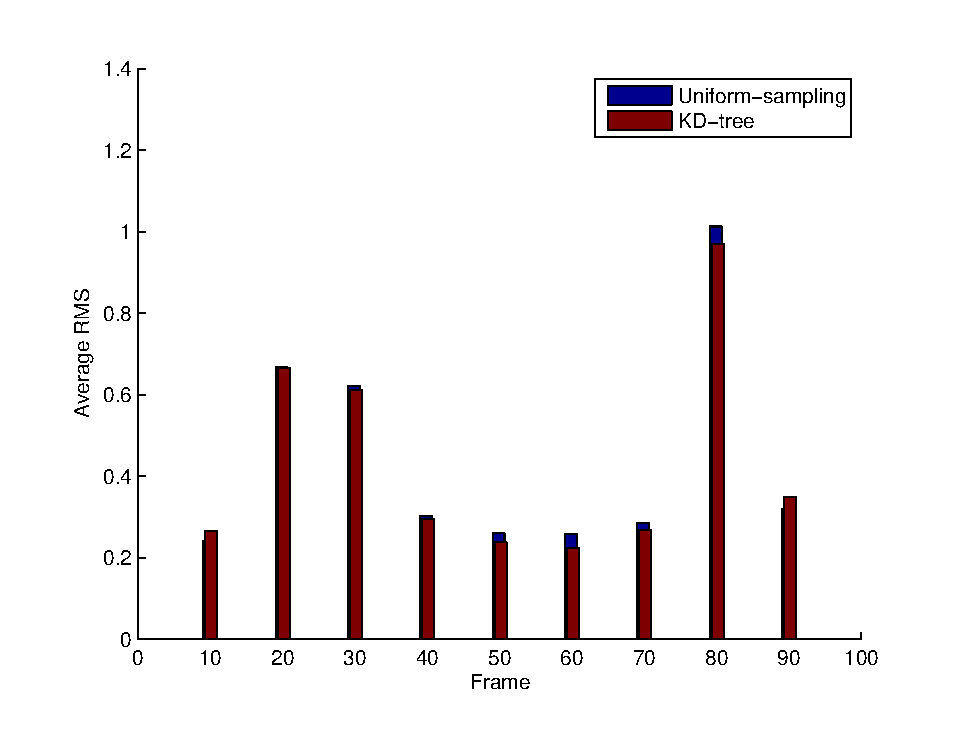
\includegraphics[width=0.48\textwidth]{figures/comparison.eps}
    \caption{RMS error comparison between KD-tree implementation and the uniform sampling.}
    \label{fig:comparison}
\end{figure}

\begin{figure}[t!]
  \centering
    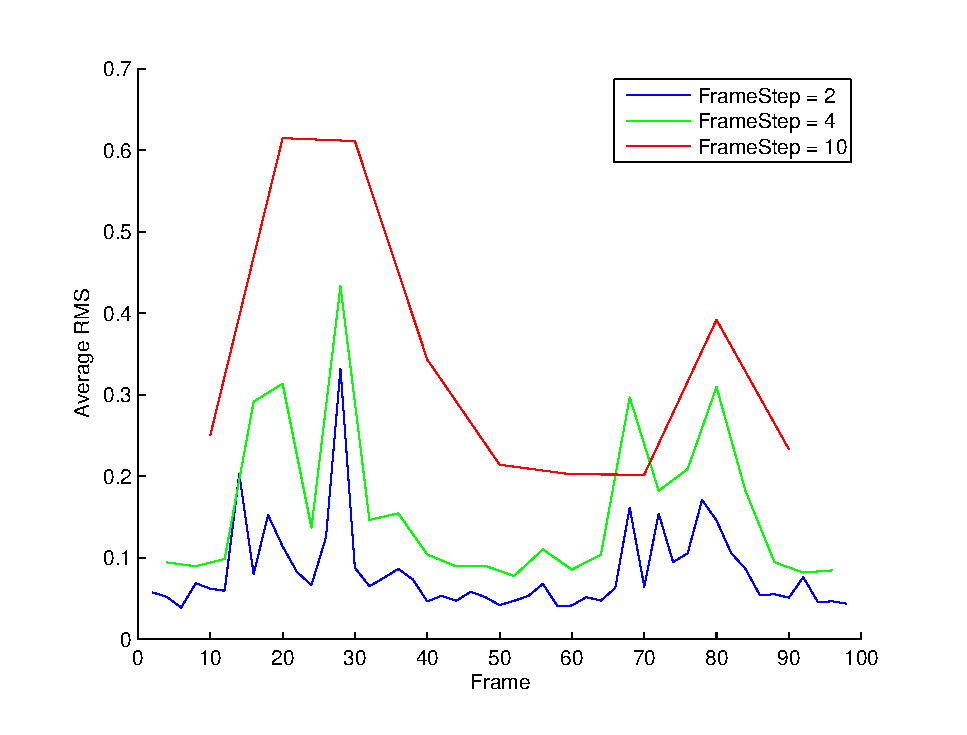
\includegraphics[width=0.48\textwidth]{figures/RMSmergedKD.eps}
    \caption{Average relative RMS error metric for merged kd-tree implementation for frame-step $1,2,4,10$.}
    \label{fig:rmsmergederror}
\end{figure}

\begin{figure}[t!]
  \centering
    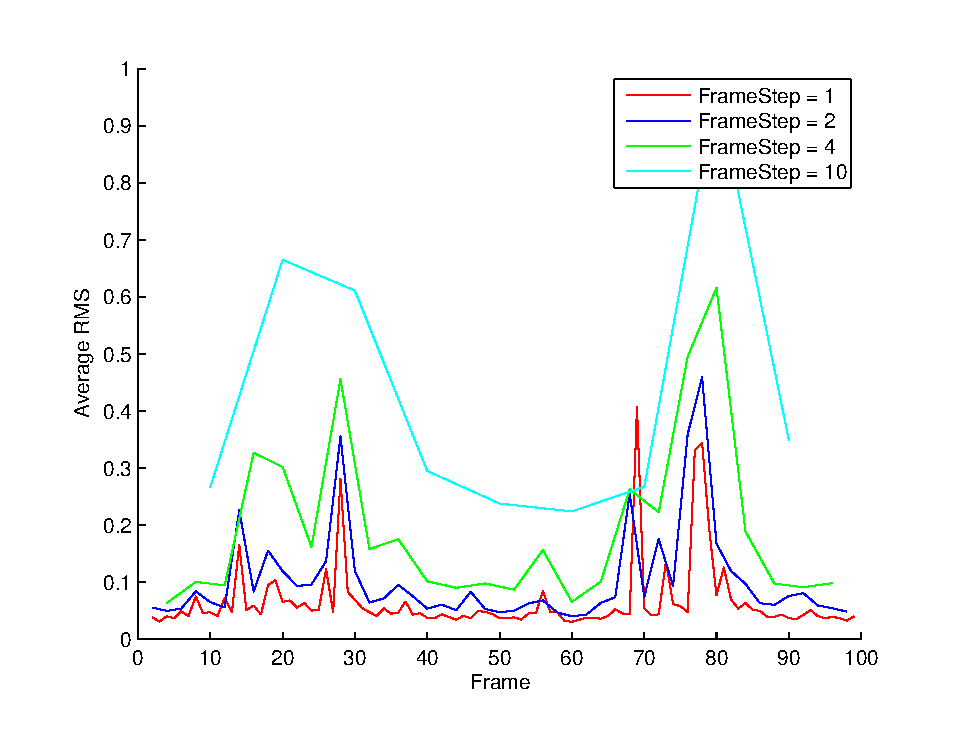
\includegraphics[width=0.48\textwidth]{figures/RMSunmergedKD.eps}
    \caption{Average relative RMS error metric for kd-tree implementation without merging for frame-step $1,2,4,10$.}
    \label{fig:rmsunmergederror}
\end{figure}

A few variants have been applied~\cite{icpVar} on the ICP algorithm, in which performance improvements resulted from different techniques for, closest point selection, point rejection and error metric variations. For point selection instead of using all available points, a uniform sub-sampling or random sampling among them can lead to faster detection of the closest points. Also, selecting points from more informative regions of the surfaces can lead to better performance since more points are needed if the gradients of the surface are of higher value. As far as matching points are concerned, we can use a few variants apart from searching the whole space of the target surface. A projection of each point in the reference surface to the target one can give us an accurate estimation about where the closest point lies. Also color and angle measurements between surfaces can give us useful information about where to find these points.

\subsection*{Dataset}
Our dataset consists of $100$ 3D point clouds that represent surfaces deriving from multiple views of a human body. 

\subsection{Implementation}
% ADD SOME EQUATIONS HERE
In order to implement our algorithm we followed the work done in ``Implementation of a 3D ICP-based Scan Matches''~\cite{icpImp}. The first and most computationally expensive step of the algorithm is to find for each point of the target cloud the closest point there is in the base one. After doing this we end up having two sets of points with size equal to the target cloud's size. These point clouds need to be centered so we can eliminate any translation the target point cloud might have. Thus, we normalize the base and target cloud's closest point sets subtracting their centers from each of their points. Applying singular value decomposition to the two normalized clouds helps us estimate the rotation of the target cloud with respect to the base. This process continues recomputing the closest points of each cloud and re-transforming the target cloud until the error is minimized.

Given the rotation, we transform the center of the target cloud by multiplying the homogeneous coordinates of it with the estimated rotation matrix subtracting it from the base cloud's center point. The resulting 3D point will serve as the translation of the target cloud with respect to the base one. Applying the estimated translation and rotation transformation onto the target cloud we acquire the new target cloud from which we can now compute the average euclidean distance from the base cloud. This process runs iteratively until the average euclidean distance is minimized.

Another important aspect of the algorithm is the way the merging of the two point clouds is done. There are two methods applied, the first is to merge the two point clouds as one and consider it as the base cloud comparing it with the next frame, and the second one is to store the merged point cloud and proceed considering the target cloud of the first iteration as the base cloud of the second.

\begin{figure*}[bt!]
  \centering
    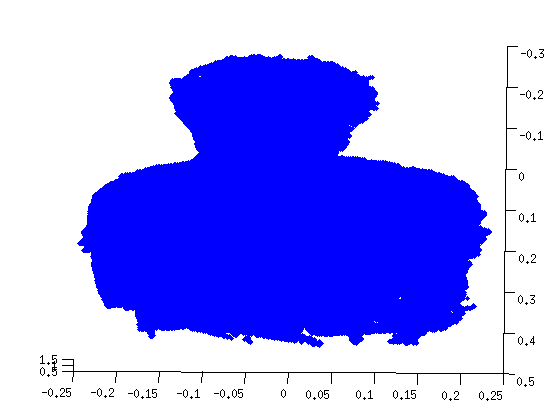
\includegraphics[width=0.24\textwidth]{figures/unBf10.png}\	
    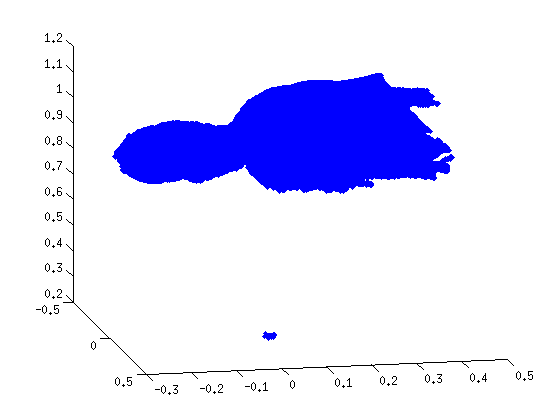
\includegraphics[width=0.24\textwidth]{figures/meUs4.png}\	
    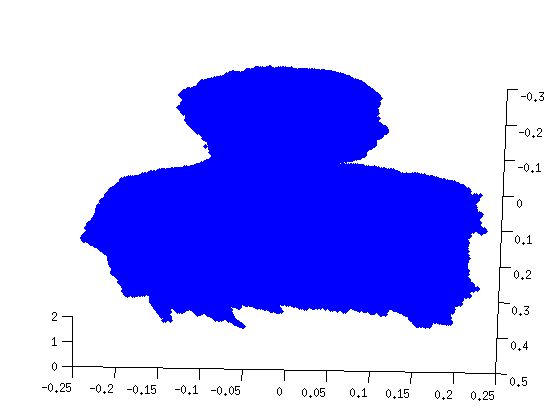
\includegraphics[width=0.24\textwidth]{figures/meKd2.png}\	
    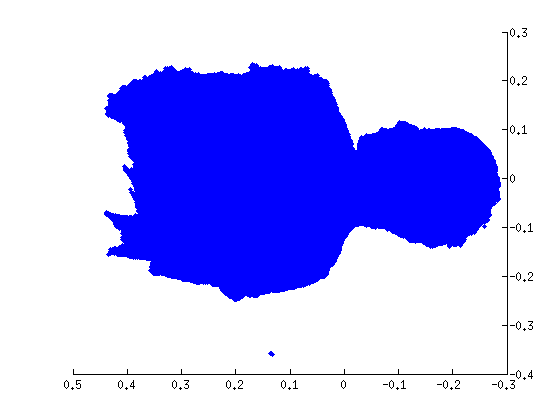
\includegraphics[width=0.24\textwidth]{figures/unKd1.png}
    \caption{Visualization of the merged pointclouds using the ICP algorithm with different closest point selection techniques. From left to right: a) brute force, frame step $10$, no merging b) Uniform sampling, frame step $4$, with merging c) KD-tree, frame step $2$, with merging d) KD-tree, frame step $1$, without merging. }
    \label{fig:mergedICP}
\end{figure*}

\subsection{Results}
We applied three different techniques for closest point selection including KD-tree, uniform sampling and brute force. Brute force searches all the points of the base for each of the target. KD-tree stores all elements of the base cloud in a KD-tree and then minimizes the complexity of finding the closest point of each target point. Uniform sampling searches the closest points of a constant number of target points using brute force again. A comparison in the error of uniform sampling and KD-tree implementation is presented in figure~\ref{fig:comparison}. In this figure we can see the average RMS error when we merge every tenth frame with the base, without merging the result in the base cloud each time.

To check also how the number of frames we skip influence the performance of the algorithm we also conducted an experiment using the KD-tree implementation for every $1,2,4,10$ frames. As we expected the error appears to be larger as we skip more frames. This result is illustrated in figure~\ref{fig:rmsmergederror} when we merge the target cloud to the base cloud in each frame. For the implementation without the merging the same results are presented in figure~\ref{fig:rmsunmergederror}.

The resulted merged surfaces are depicted in figure~\ref{fig:mergedICP}. There we can see the merged point clouds that represent the connected point clouds thought the sequence in the database.


\subsection{Discussing the ICP algorithm}
Using the estimated camera poses, merge the point-clouds of all the scenes into one point-cloud and visualize the result. Does the merging produce sufficient result? Discuss why. Now, estimate the camera pose and merge the results using every 2 nd , 4 th , and 10 th frames. Does the camera pose estimation change?




So the estimated camera poses change in comparison with the previous estimates (Sec- tion 2.1)? Does this estimation produce better results?

Even though the ICP algorithm produces sufficient results for surface registration it still has major drawbacks when it comes to its computational cost which makes it really time demanding. The techniques presented earlier in this section improve its complexity without harming the performance. Another issue that arises when it comes to the performance of the algorithm is the fact that the surfaces to be merged need to be close to each other in terms of camera viewpoint, so the merging will converge to a quality solution.

2. How do you think the ICP algorithm can be improved, beside the techniques mentioned in [2], in terms of efficiency and accuracy?



\section{Epipolar Geometry and Chaining}
\label{egc}
In this section we are going to describe the first part of the Structure from Motion algorithm, which is to exploit prior knowledge about the scene. This is done by finding corresponding image points in multiple views and compute their epipolar geometry which is expressed algebraically by the fundamental matrix which can be decomposed to obtain the required projection matrices.

\subsection{Dataset}
The data we were required to use consists of two individual datasets. The first one contains 49 frames, each one of them depicting a house from a different angle. The second contains 16 frames, each one of them depicting a teddy-bear from a different view. In each frame, there is a slight movement of the target object with respect to the previous frames.

\subsection{Implementation}
An important step of the algorithm is to identify local features in each image which are consistent in most of the frames. For this purpose we used the  Scale-Invariant Feature Transform (SIFT) (vl\_ sift function in vlFeat library) algorithm to detect points of interest in each frame. In order to restrict the search process of the SIFT detector an active contour based segmentation was used. By applying this technique we were able to segment the frames into background and foreground regions, allowing us to focus only on the points that exist on the object of interest as presented in figure~\ref{fig:houseBackground}.

\begin{figure}[ht!]
  \centering
    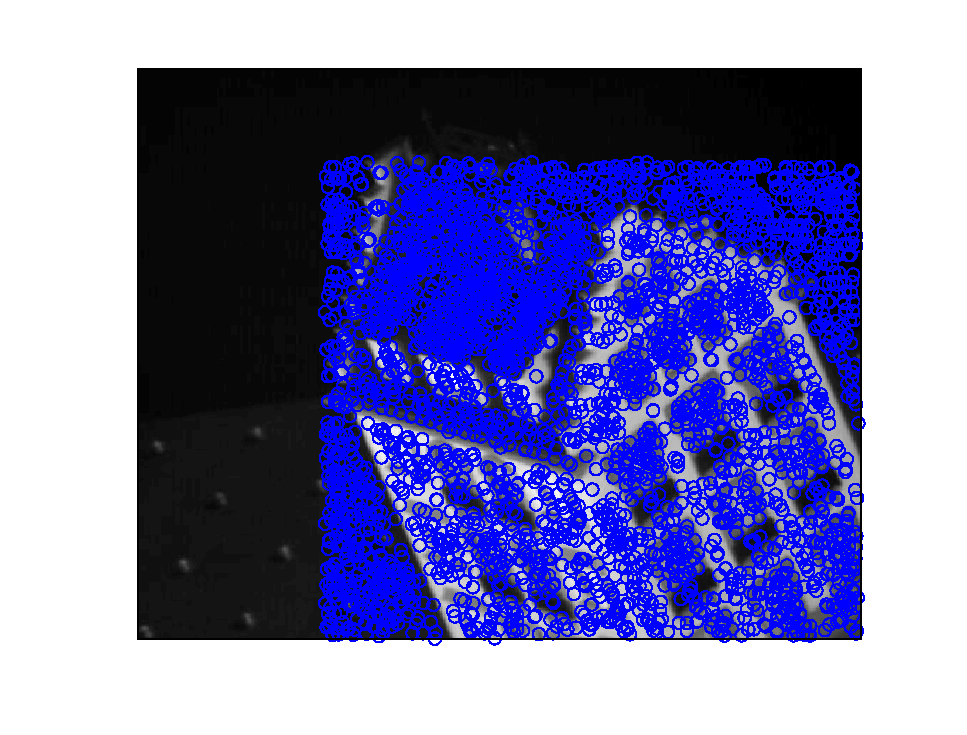
\includegraphics[width=0.49\textwidth]{figures/houseBackground.eps}
    \caption{Feature points extracted by the SIFT detector found on the object of interest}
    \label{fig:houseBackground}
\end{figure}

By finding feature points in every frame we are able to identify matches in consecutive frames. This is done by using the built-in function vl\_ ucbmatch of the vlFeat library of MATLAB which returns the qualitative corresponding feature points and rejects the ambiguous ones. The vl\_ sift command without parameter tuning gives only a limited number of feature points as illustrated on the first image of figure~\ref{fig:matches}. By setting a higher edge threshold which serves to filter out edge-like features we were able to obtain more key points. Another parameter we tuned was the number of levels per octave. By increasing this number in principle it returns more refined keypoints, but in practice the selection may be unstable due to noise. Feature matches between two consecutive frames of the House dataset with tuned parameters, are displayed on the second image of figure~\ref{fig:matches}.

\begin{figure}[ht!]
  \centering
    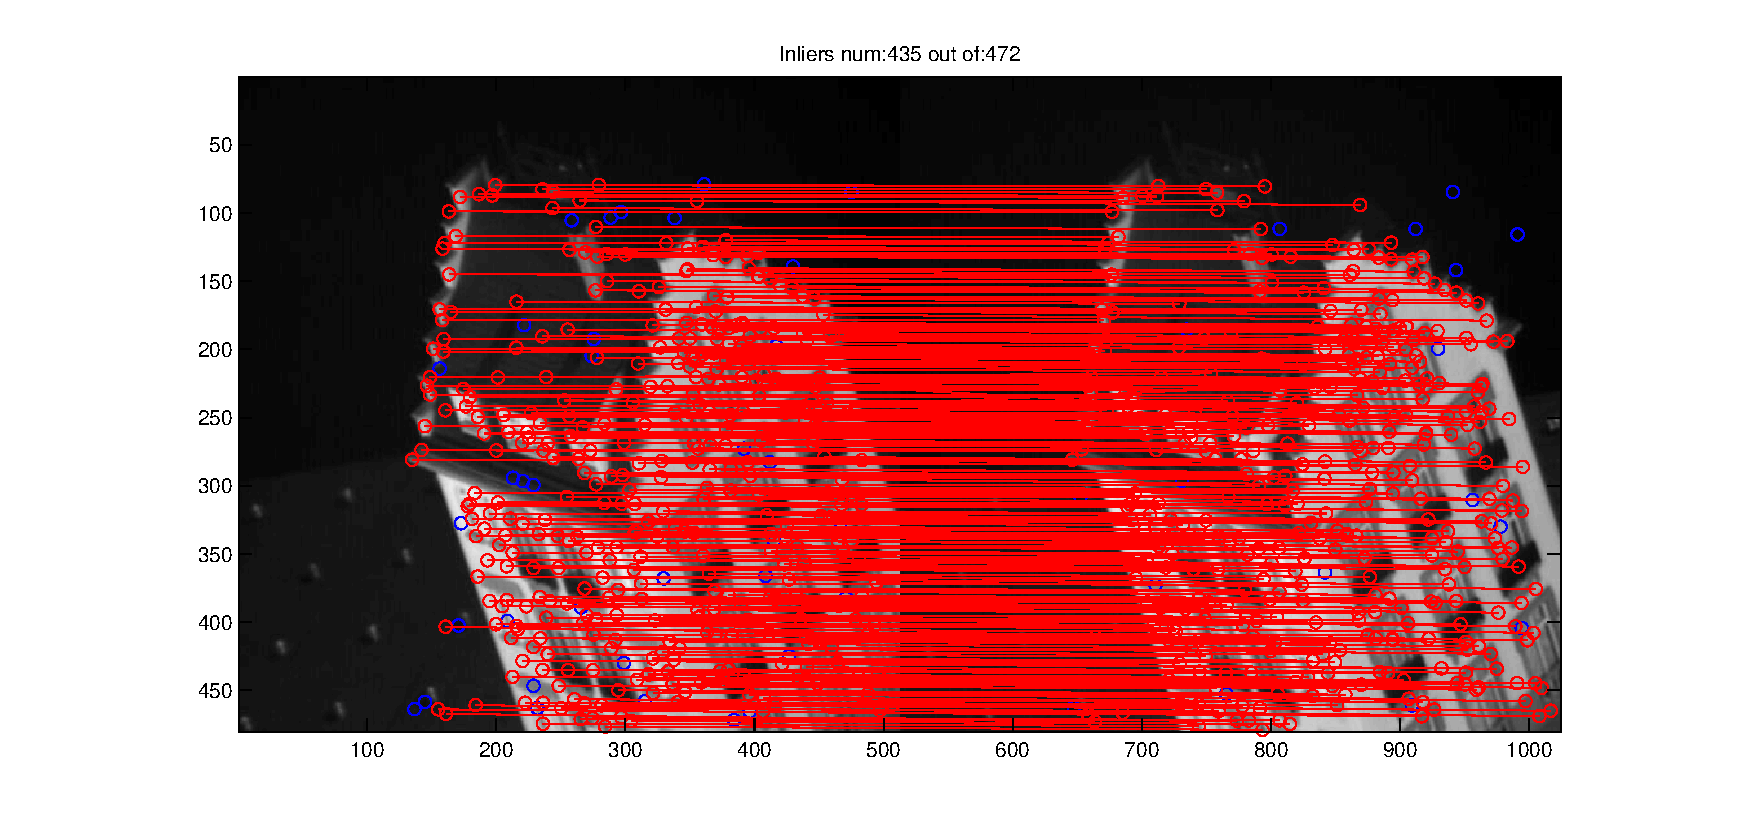
\includegraphics[width=0.55\textwidth]{figures/matchesSimple.eps}\\
    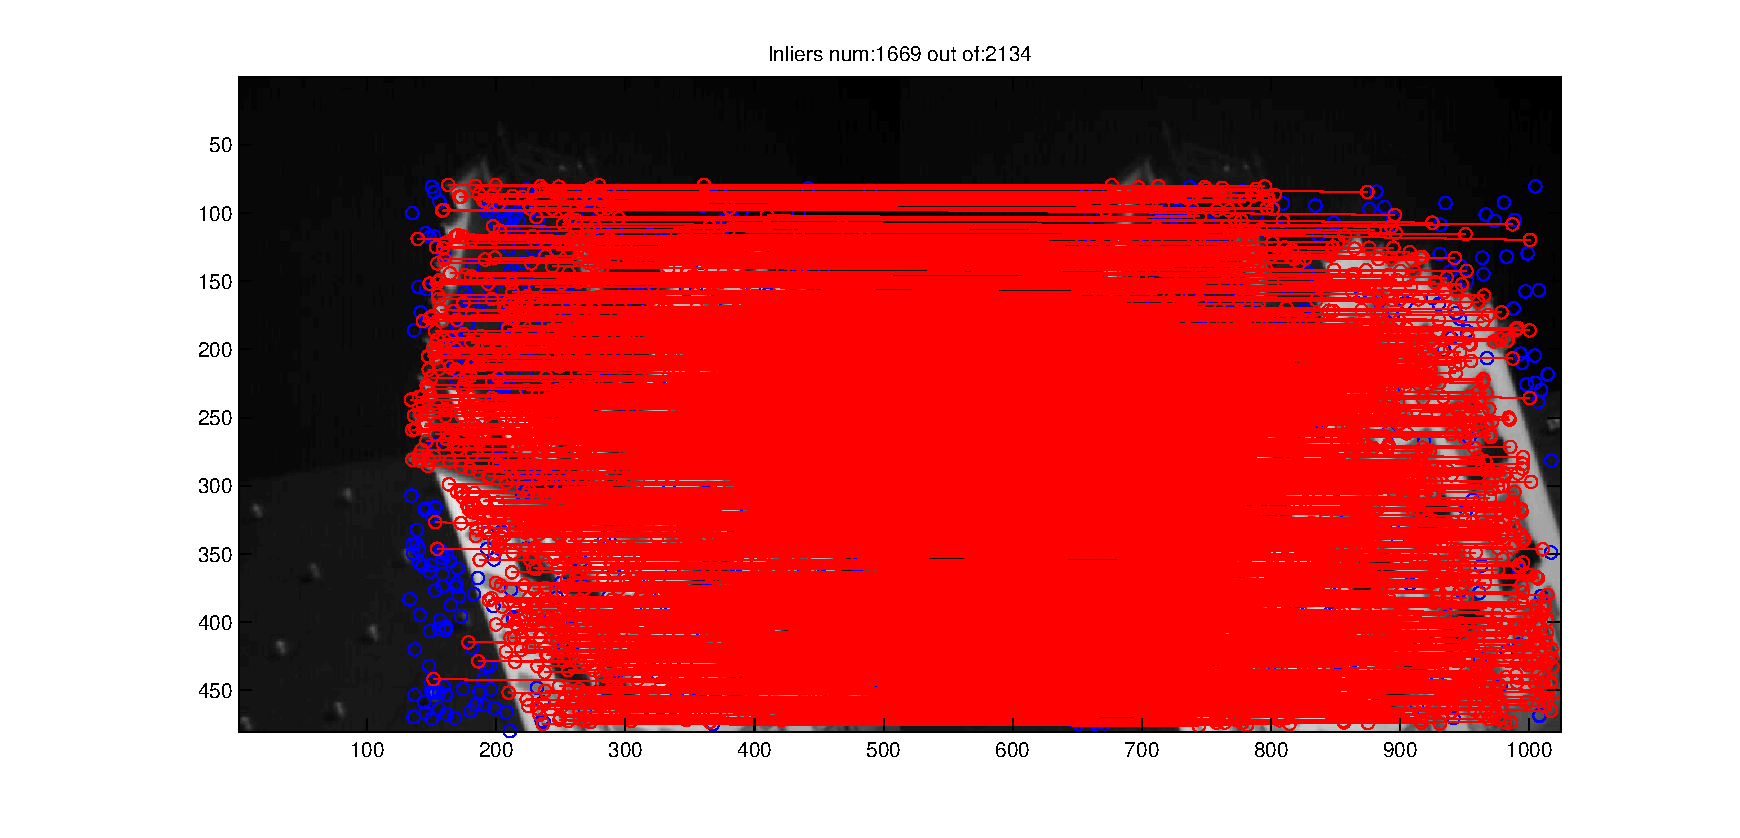
\includegraphics[width=0.55\textwidth]{figures/matchesWithThresh.eps}
    \caption{Above: Feature matches between two consecutive frames without tuned parameters, Below: Feature matches between two consecutive frames with parameter tuning: edgeThresh: 30, Levels: 30.}
    \label{fig:matches}
\end{figure}

The next step is to apply centering to the points, namely subtract the centroid of the feature points (remove translation) according to :

\begin{equation}
\hat{x} = x_{ij} - \frac{1}{n} \sum_{k=1}^{n} x_{ik}
\end{equation}

To estimate the fundamental matrix deriving from the corresponding image points extracted by the SIFT detector the normalized Random Sample Consensus (RANSAC) eight-point algorithm~\cite{eight-point} was implemented. Application of this algorithm leads to a more stable result than the simple eight-point implementation. The steps of the algorithm are:

\begin{enumerate}[1]
  \item Pick 8 random matches from the list of the corresponding points.
  \item Construct a matrix A from the matches and get the transformation matrix from the last column of V of the Singular Value Decomposition of A.
  \item Count the number of inliers (points that agree with the transformation matrix) by computing the Sampson distance (if distance is smaller than a certain threshold then we consider the point as an inlier)
  \item Repeat steps 1 to 3 until the majority of the points are inliers.
\end{enumerate}


\subsection{Chaining}
The last step is to construct the Point View Matrix which contains normalized point coordinates (inliers). Actually it is not always the case that many points are present in all frames due to the fact that the frames may have considerably large difference in view among them. In figure~\ref{fig:pointMatching} the feature point view matrices for the house and teddy-bear datasets are illustrated. We can see that the teddy-bear dataset produces a vastly more sparse point view matrix compared to the one the house dataset produces. These point view matrices will be used in the $2^{nd}$ part of the SFM implementation, in order to build a 3D structure of these two objects.

\begin{figure}[ht!]
  \centering
    \includegraphics[width=0.50\textwidth]{figures/pvmList.eps}
    \caption{Point view matrix sequences, Horizontal axis denotes detected feature points, vertical axis are the frames. Lines starting from the top going to the bottom of the picture represent points detected in consecutive frames.}
    \label{fig:pointMatching}
\end{figure}


\section{Structure from Motion}
\label{sfm}

The last part of the lab assignment discusses the final parts of the Structure from Motion (SFM) algorithm. In particular, using the output of the assignment's $2^{nd}$ part, we derive the motion and shape matrix of a given set of points.  

\subsection{Implementation Details}
As mentioned above, the data used by this part of the algorithm is an $m\times n$ matrix, where $m$ is the total number of frames, and $n$ is the total number of feature points extracted by the previous step of SFM. 
Given this "Point View" matrix, we gather feature points that persist through a sufficient number of frames, and construct a new $A: 2m\times n'$ matrix, where each row represents a 2D coordinate of each of $n'$ feature points. Note that this matrix is dense enough to adequately describe 3D structure given 2D feature points.

After obtaining matrix $A$, 3D coordinates must be calculated for each feature point, with respect to every frame. In order to achieve that, we need to normalize the 2D coordinates in $A$. For each row of the $A$ matrix, we calculate the centroid (the average coordinate over all feature points) which then we subtract from every point coordinate in the same row. By doing this, we relate every feature point to a 3D position in the resulting 3D structure.

Following normalization, SVD is applied to the (normalized) $A$ matrix to obtain the motion \& shape matrices:  
$D = U\times W\times V^T$

We need to reduce the rank of the resulting matrices to 3, in order to obtain 3D coordinates, so we use the 3 first columns of $U$, the 3 first rows of $V^T$ and the top-left $3\times 3$ matrix of $W$ to obtain $U_3, W_3,$ and $V^T_3$. Lastly, the matrix \& shape functions are given by: $M = U_3W^{\frac{1}{2}}_3$, $S = W_3^{\frac{1}{2}}V^T_3$

\subsection{Dealing with affine ambiguity}
The process described before, implies a decomposition that is subject to affine transformation\cite{amb}. Taking that into account, we further factorize matrices $M\rightarrow \hat{M}$ \& $S\rightarrow \hat{S}$ according to Morita and Kanade (1997)\cite{amb}. In more detail, we calculate matrix $A^{-1}$ and $A$ where $A$ represents an affine transform that transforms $\hat{M}$ into $M$ and $A^{-1}$ transforms $\hat{S}$ into $S$. Applying these matrix manipulations erases the affine ambiguity, under the assumption that image axes must be perpendicular\cite{amb}.

Looking at figures ~\ref{fig:icp4-11-Amb} and ~\ref{fig:icp4-11}, we can se that the latter has a slightly better structure, as far as the position and distance between feature points is concerned. 

\subsection{Frame sampling}
We have observed that many feature points are detected at non-informative positions, implying a noise factor in our SFM implementation. In order to reduce the noise, while also increasing the speed of the algorithm, we sampled though the frame set, by skipping 1, 2, 4, 5 or 8 frames. In the results section we can see how this parameter changes the 3D structure, and conclusions on it are derived in the discussion section.


\subsection{Results}

Below, we present the results obtained by the SFM implementation. 

\begin{figure}[ht!]
  \centering
    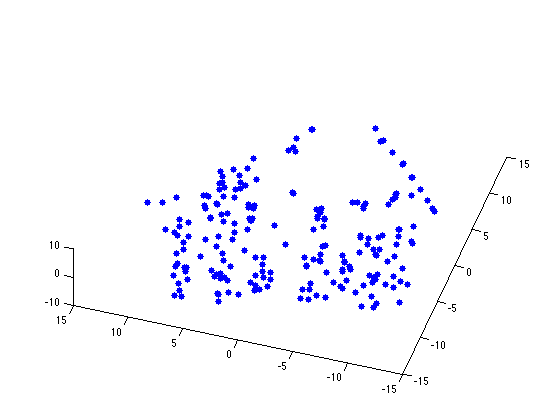
\includegraphics[width=0.49\textwidth]{figures/icp1-46-Amb.png}
    \caption{3D structure of the house frameset, sampling all frames, without affine ambiguity correction.}
    \label{fig:icp1-46-Amb}
\end{figure}

\begin{figure}[ht!]
  \centering
    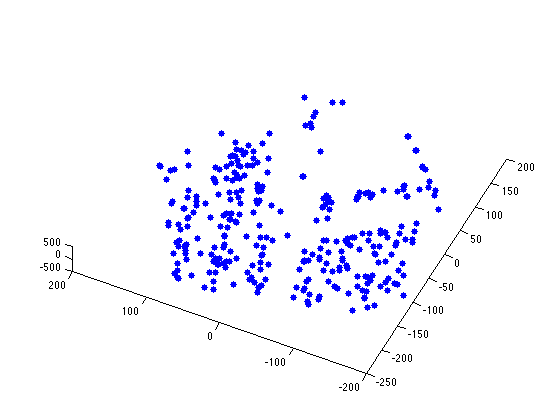
\includegraphics[width=0.49\textwidth]{figures/icp2-22.png}
    \caption{3D structure of the house frameset, sampling every 2 frames, with affine ambiguity correction.}
    \label{fig:icp2-22}
\end{figure}


\begin{figure}[ht!]
  \centering
    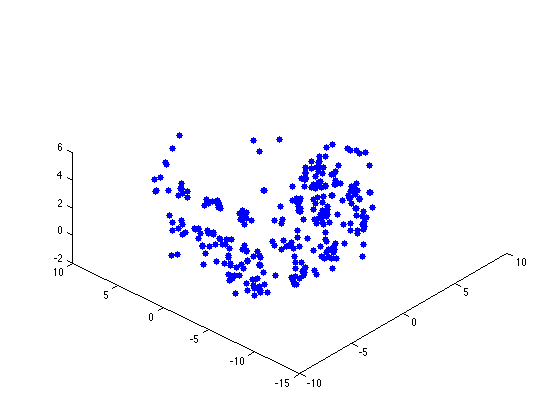
\includegraphics[width=0.49\textwidth]{figures/icp4-11-Amb.png}
    \caption{3D structure of the house frameset, sampling every 4 frames, without affine ambiguity correction.}
    \label{fig:icp4-11-Amb}
\end{figure}

\begin{figure}[ht!]
  \centering
    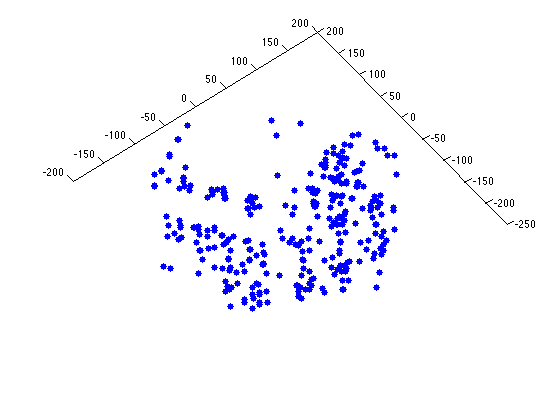
\includegraphics[width=0.49\textwidth]{figures/icp4-11.png}
    \caption{3D structure of the house frameset, sampling every 4 frames, with affine ambiguity correction.}
    \label{fig:icp4-11}
\end{figure}

\begin{figure}[ht!]
  \centering
    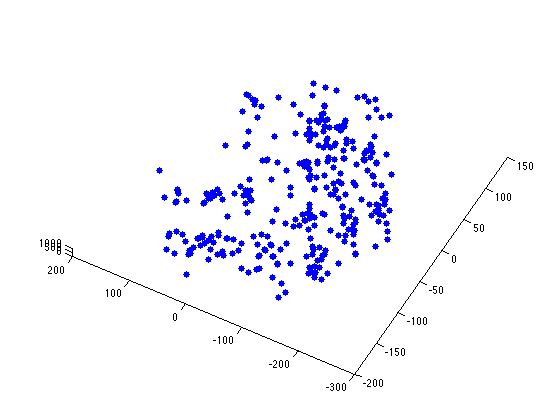
\includegraphics[width=0.49\textwidth]{figures/icp5-8.png}
    \caption{3D structure of the house frameset, sampling every 5 frames, with affine ambiguity correction.}
    \label{fig:icp5-8}
\end{figure}

\begin{figure}[ht!]
  \centering
    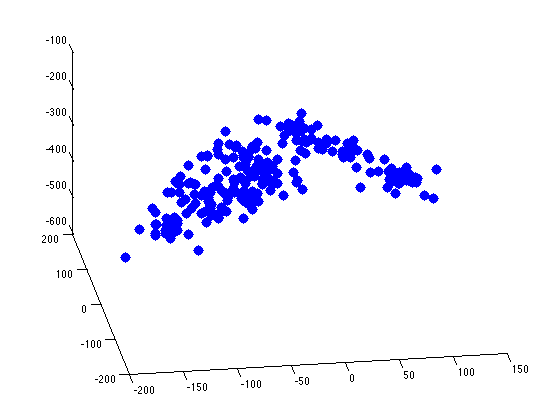
\includegraphics[width=0.49\textwidth]{figures/icp8-5.png}
    \caption{3D structure of the house frameset, sampling every 8 frames, with affine ambiguity correction.}
    \label{fig:icp8-5}
\end{figure}



\subsection{Discussion}
This last step of the SFM algorithm gave us the opportunity to observe the results in practice. Given a set of frames, we used SFM to construct a 3D model of the object presented. 

However, while experimenting with two different sets of frames (House \& Teddybear), we discovered that the teddybear frameset is not capable of producing an efficient 3D model, while the house frameset does. An explanation to why this happens lies not in the actual implementation of the algorithm, but the dataset itself. It is a fact that the teddybear frameset contains a 360 degree y-axis rotation of the object, resulting in significantly less feature points being persistent through a large number of frames. 
On the other hand, the house frameset does not contain such steep change in point of view, but only a slight z-axis rotation. As a result, the number of feature points detected in all frames is higher, thus, the 3D model reconstructed by SFM looks more realistic.

Furthermore, regarding the frame sampling feature introduced, we can observe an improvement between figure ~\ref{fig:icp1-46-Amb} and figure ~\ref{fig:icp4-11-Amb}, in terms of how realistic the structure looks. We can see that many new feature points are introduced, while in figure ~\ref{fig:icp4-11}, almost no noisy points are present.

Despite the improvement achieved, we can observe in figures ~\ref{fig:icp5-8} and ~\ref{fig:icp8-5} that sparse sampling can lead to undesired results. The structure of the house is inconsistent, especially in figure ~\ref{fig:icp8-5} where only feature points on the house roof are detected in all sampled frames. 

\section{Printable 3D Model}

We were assigned with the task of structuring a triangular watertight mesh, given a 3D point cloud representing a human.
Figure ~\ref{fig:sundin-pointcloud} represents a visualization of this point cloud.
\begin{figure}[ht!]
  \centering
    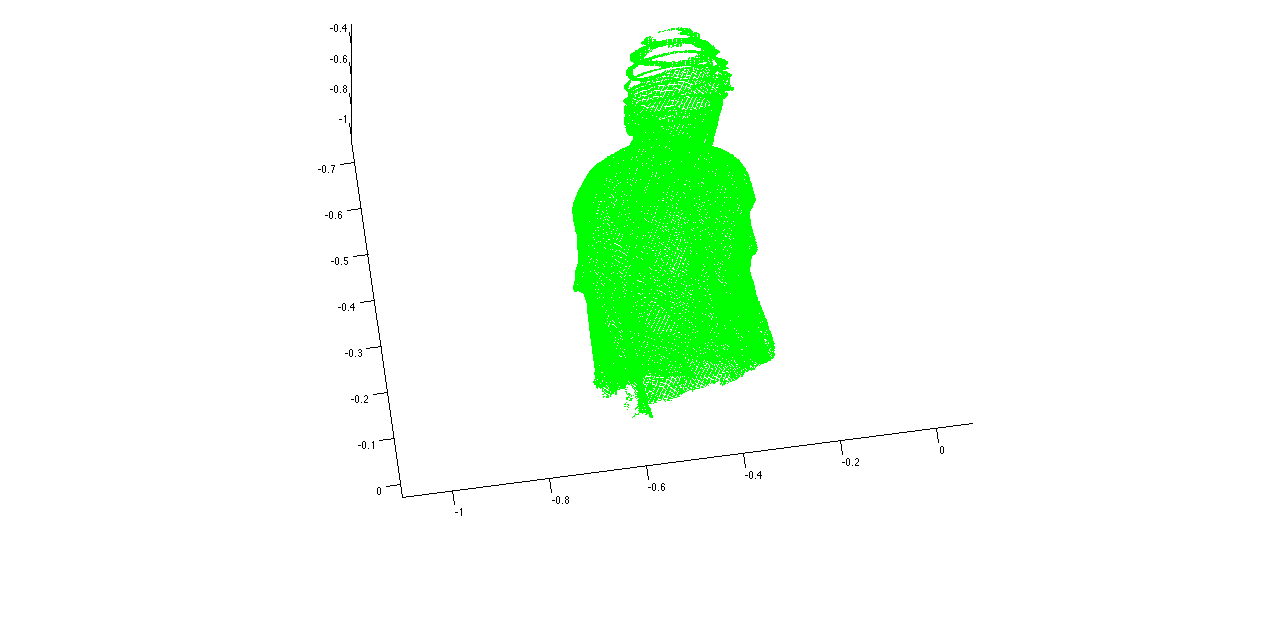
\includegraphics[width=0.49\textwidth]
    {figures/pointCloud_sundin.png}
    \caption{Visualization of a 3D point cloud of a human}
    \label{fig:sundin-pointcloud}
\end{figure}


\subsection{PCL (C++)}
In order to build a printable 3D model given a point cloud, we used the Point Cloud Library (PCL)\cite{pcl}. PCL has built-in functions in order to read and visualize a 3D point cloud using triangulation. 

\subsection{MyCrust (MATLAB)}
In order to visualize a 3D point cloud in MATLAB, we used the "myCrust.m" toolbox. The functions it supplies construct a triangular mesh given a point cloud as input. In order to retrieve the data, we used the given readPcd() function, while we also used the MATLAB built-in function imfill() to create a watertight model. The latter function will "fill the holes" of every plane in the whole dataset. 

Snapshots of the visualization are presented in the section below.
\subsection{Results} 




\begin{figure}[ht!]
  \centering
    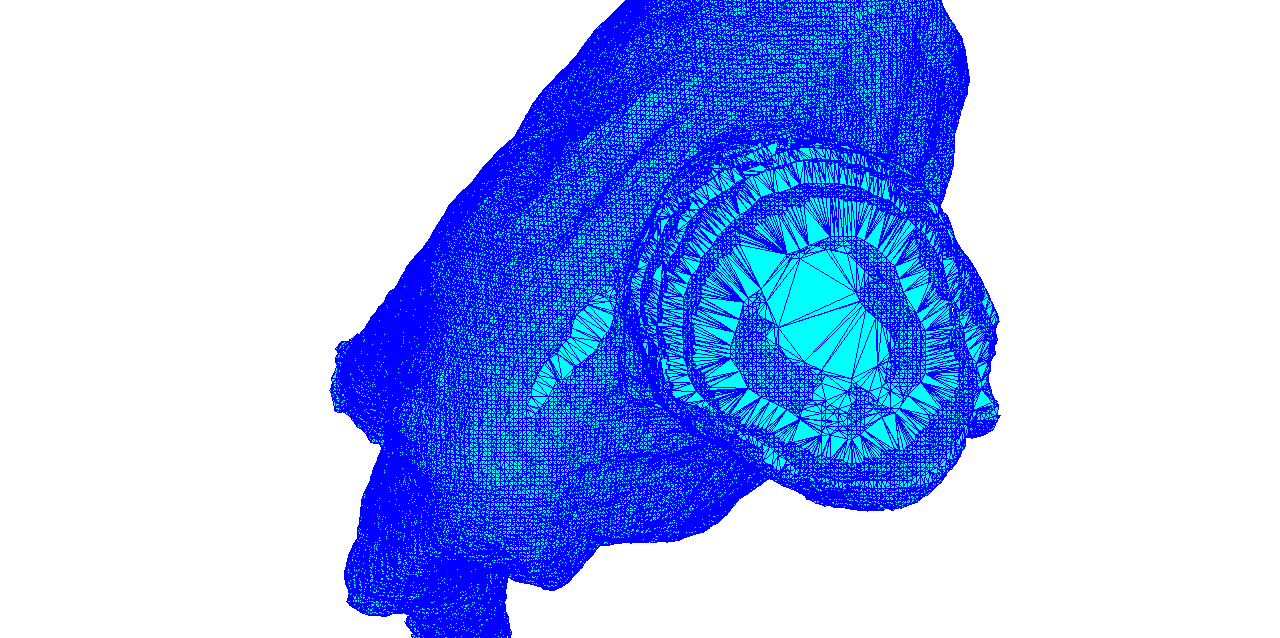
\includegraphics[width=0.49\textwidth]{figures/3dMesh_sundin_zoom_top.png}
    \caption{Printable triangular mesh, top view}
    \label{fig:sundin-top-zoom}
\end{figure}

\begin{figure}[ht!]
  \centering
    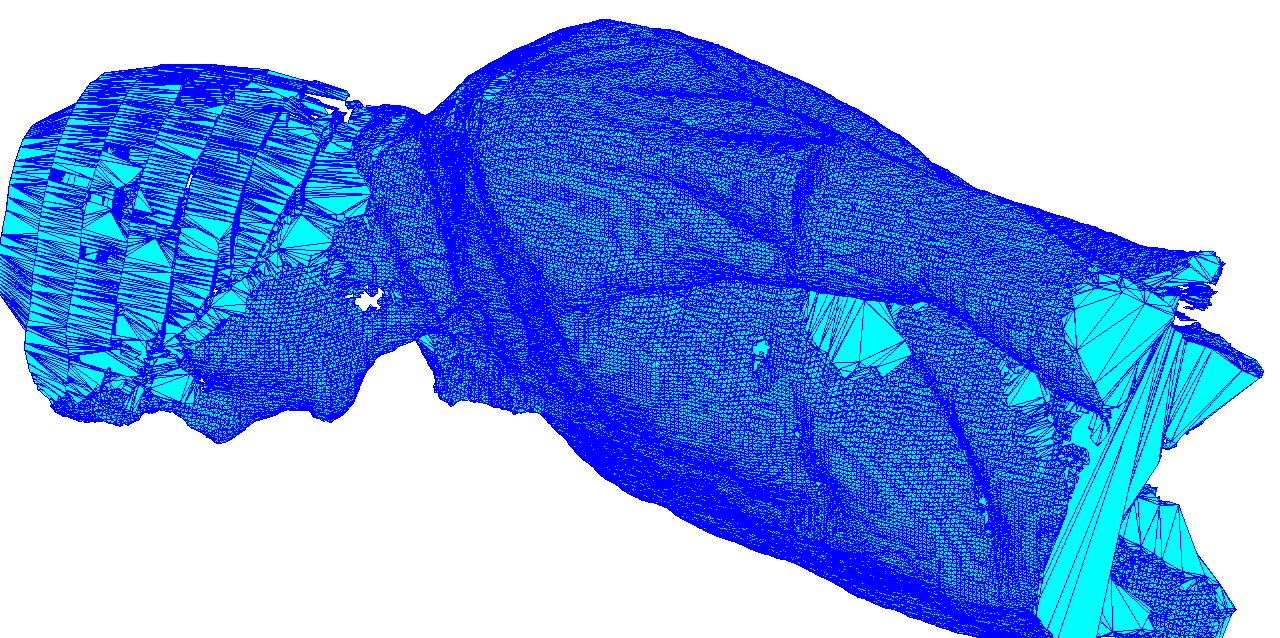
\includegraphics[width=0.49\textwidth]		{figures/3dMesh_sundin_zoom_side.png}
    \caption{Printable triangular mesh, side view}
    \label{fig:sundin-top-zoom}
\end{figure}

\begin{figure}[ht!]
  \centering
    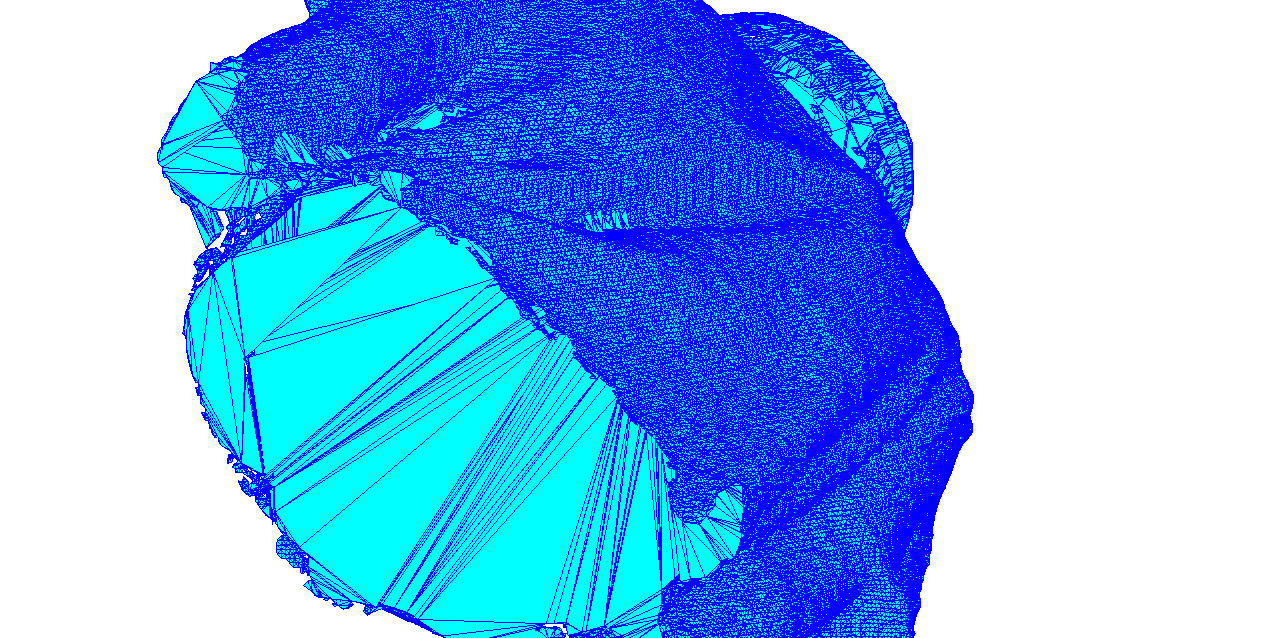
\includegraphics[width=0.49\textwidth]{figures/3dMesh_sundin_zoom_bot.png}
    \caption{Printable triangular mesh, bot view}
    \label{fig:sundin-top-zoom}
\end{figure}




\section{Conclusion}
\label{conclusion}


\begin{thebibliography}{9}

\bibitem{pcl}
Radu Bogdan Rusu and Steve Cousins, "3D is here: Point Cloud Library (PCL)", IEEE International Conference on Robotics and Automation (ICRA), May 9-13 2011.

\bibitem{myc}
Luigi Giaccari, MyCrust.m toolbox,
http://www.codeforge.com/read/218867/MyCrust.m__html

\bibitem{icp}
Besl, Paul J., and Neil D. McKay. ``Method for registration of 3-D shapes.'' In Robotics-DL tentative, pp. 586-606. International Society for Optics and Photonics, 1992.

\bibitem{egc}
Rothganger, Fred, Svetlana Lazebnik, Cordelia Schmid, and Jean Ponce. ``3d object modeling and recognition using local affine-invariant image descriptors and multi-view spatial constraints.'' International Journal of Computer Vision 66, no. 3 (2006): 231-259.

\bibitem{eight-point}
Richard I. Hartley. ``In Defence of the 8-point Algorithm.'' (1997)


\end{thebibliography}

\end{document}
